\documentclass[12pt, conference]{IEEEtran}

%\usepackage[margin=0.5in]{geometry}
\usepackage{multicol}
\usepackage{cite}
\usepackage{graphicx}
\usepackage{amsmath}
\usepackage{amsthm}
\usepackage{subcaption}
\usepackage{setspace}

\onecolumn

\begin{document}

	\title{Bottlenecked Function Prediction Using NNs}
	\author{Yuval Alfassi}
	\date{March 2020}
	\maketitle


    \begin{spacing}{1.5}

		\section{Objective}
			Given the multidimensional function $F(x_1,x_2,x_3,x_4) = (x_1+x_2)^2+(x_2+x_4)^2$, are there functions $g_1,g_2,h$ such that $h(g_1(x_1,x_3),g_2(x_2,x_4)) = F(x_1,x_2,x_3,x_4)$ (where $h$ is a second degree polynomal and $g_1$,$g_2$ are linear)?

			Let's try that with Neural Networks!
		\section{Test Data}
			$x_1,...,x_4$ were sampled out of $[0,2]$. $1000$ point samples were generated randomly (uniform distribution). The distribution of the points in regard to $F$ is as follows:
			\begin{center}
				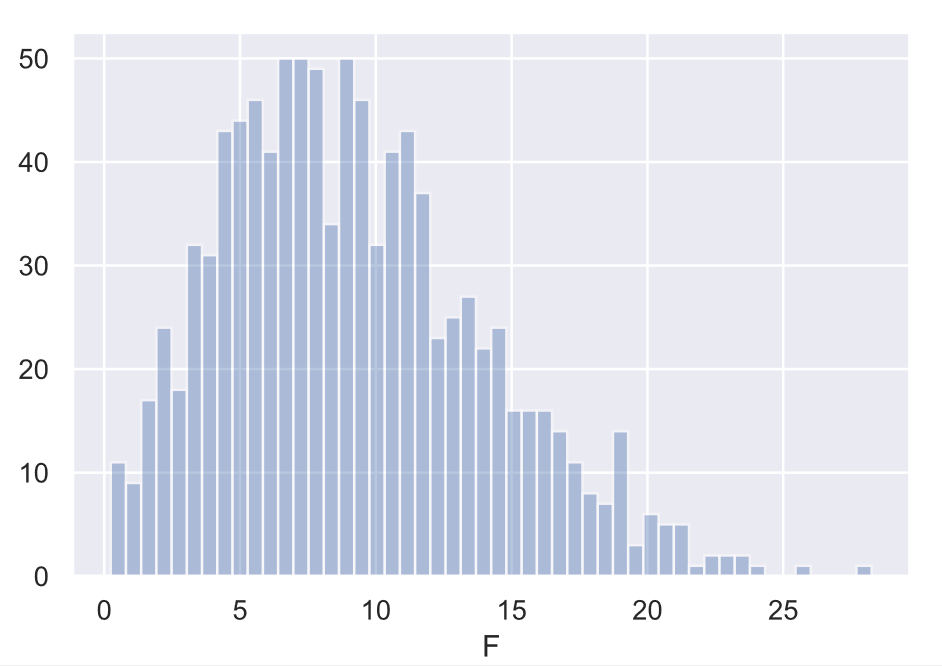
\includegraphics[width=0.5\textwidth]{Figures/points_distribution.png}
			\end{center}
			The NNs were trained using only these points as a train set. No test set or validation set are required.

		\section{Fully Connected NN}
			A fully connected NN with a dense architecture of $4\times10\times10\times1$ converges very fast. It's predictions are:
			\begin{center}
				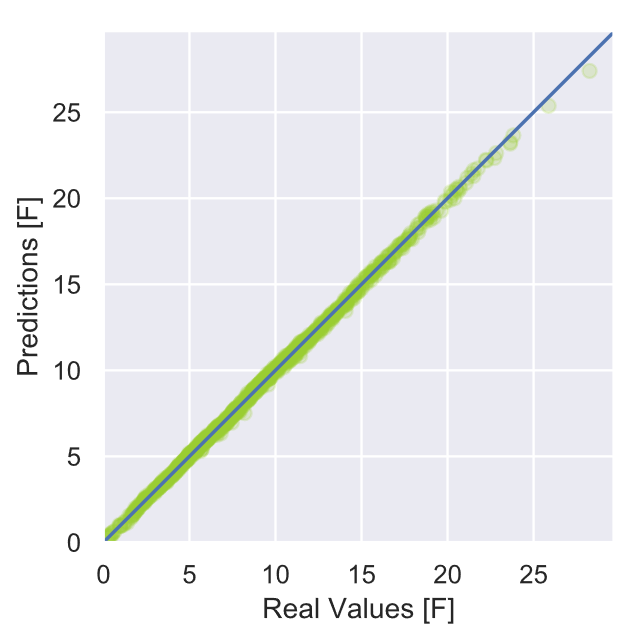
\includegraphics[width=0.5\textwidth]{Figures/fully_nn_predictions.png}
			\end{center}
			The MSE of the predictions is \textbf{0.017}.

		\section{$\{x_1,x_2\},\{x_3,x_4\}$ Function Partition}
			Now, lets divide the input points of $F$ into: $h(g_1(x_1,x_2),g_2(x_3,x_4)) = F(x_1,x_2,x_3,x_4)$.
			For that, the NN has to be 'halved', so two NN architechtures with $2$ input neurons merge into a big NN.
			The NNs are of size $2\times1$ which then merge into a dense NN of $2\times6\times6\times1$.
			The predictions are:
			\begin{center}
				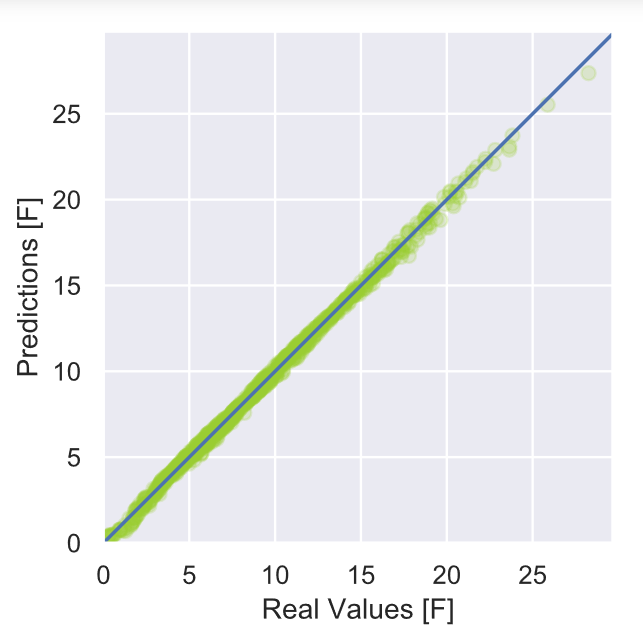
\includegraphics[width=0.5\textwidth]{Figures/bottlenecked_nn_good_partition.png}
			\end{center}
			The MSE of the predictions is \textbf{0.021}.
		
		\section{$\{x_1,x_3\},\{x_2,x_4\}$ Function Partition}
			The more interesting way to divide the input is $\{x_1,x_3\},\{x_2,x_4\}$, i.e. see whether $h,g_1,g_2$ exist s.t $h(g_1(x_1,x_3),g_2(x_2,x_4)) = F(x_1,x_2,x_3,x_4)$.
			The same NN architecture as before was used.
			The predictions are:
			\begin{center}
				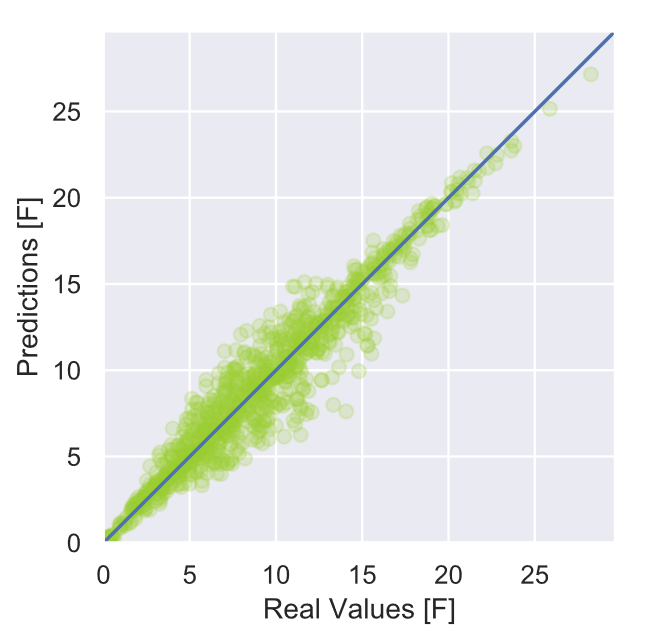
\includegraphics[width=0.5\textwidth]{Figures/bottlenecked_nn_bad_partition.png}
			\end{center}
			The MSE of the predictions is \textbf{1.81}.
			
			Unfortanately, deeper NNs do not converge, and wider NNs do not yield better results
    \end{spacing}
    
\end{document}